\begin{ParaColumn}[\bisection*{Analysis and Discussion}{分析与讨论}]

    \switchcolumn[0]*[\biparagraph{Shear Strength}{抗剪强度}]

    \enautoref{figure:2}(b) presents shear strength for all tests collected in terms of the maximum friction angle ($\phi_{\max}$) against the effective normal pressure on the failure plane ($\sigma_n^\prime$), according to the Mohr-Coulomb failure criterion. \enautoref{figure:2}(b) also includes the limits for high, average and low shear strength proposed by \citet{Leps19701159} and \citet{Indraratna1994539}, which can be expressed as:

    \switchcolumn

    \cnautoref{figure:2}(b)给出了根据Mohr-Coulomb破坏准则以最大摩擦角($\phi_{\max}$)相对于破坏平面上的有效法向压力($\sigma_n^\prime$)收集的所有试验的剪切强度。 \cnautoref{figure:2}(b)还包括\citet{Leps19701159}和\citet{Indraratna1994539}提出的高,平均和低剪切强度的限值,可以表示为:

    \CrossColumnText{
        \begin{align}
            \phi_{\max}=-2.8\ln\sigma_n^\prime+\phi_1
            \label{equation:1}
        \end{align}
    }

    \switchcolumn*

    \noindent
    with $\sigma_n^\prime$ in MPa and $\phi_{\max}$ in degrees; and $\phi_1$ = maximum friction angle at $\sigma_n^\prime=1.0$ MPa, and is 36°, 41°, and 46° for low, average, and high strength according to \citet{Leps19701159}, respectively, and 33° for the low strength limit proposed by \citet{Indraratna1994539}.

    \switchcolumn

    \noindent
    $\sigma_n^\prime$以MPa为单位,$\phi_{\max}$以度为单位; $\phi_1$在$\sigma_n^\prime=1.0$ MPa时取最大值,根据\citet{Leps19701159}的标准,低,中,高强度分别对应为36°,41°和46°,\citet{Indraratna1994539}建议的低强度极限分别为33°。

    \switchcolumn*

    For rockfills, ballasts, and sands, \enautoref{figure:2}(b) confirms that shear strength decreases with $\sigma_n^\prime$, as a consequence of dilatancy decreasing due to particle rearrangement and crushing. At the highest stress levels presented, no constant critical friction angle could be observed, which can be attributed to significant particle crushing potential still relevant at higher strains \citep{Coop2004157}, compared to limited maximum strains of 15$\%$ to 20$\%$ in triaxial testing. While common values of $\phi_{\max}$ in dense sands at low confining pressure are typically between 40° and 45° \citep{Bolton198665,Biarez19941,Schanz1996145}, all rockfills in \enautoref{figure:2}(b) present $\phi_{\max}>45^\circ$ at $\sigma_n^\prime<0.2$ MPa, due to the interlocking of highly angular grains and high friction on the rough surfaces of crushed rocks. This effect is even more significant in ballast materials, where $\phi_{\max}$ reaches values higher than 60° at low stresses. At $\sigma_n^\prime>0.5$ MPa, $\phi_{\max}$ in rockfills and ballasts decreases to values between 35° and 45°, approaching the results reported in dense sands. In general, the shear strength of quartzitic sands stays below the average values for rockfills, near the low strength limit proposed by \citet{Leps19701159} (i.e., $\phi_1=36^\circ$). For $\sigma_n^\prime<0.7$ MPa, the low shear strength limits proposed by \citet{Leps19701159} and \citet{Indraratna1994539} seem conservative for rockfills and ballasts. Therefore, a new low strength limit is proposed here for low stress, given by:

    \switchcolumn

    对于碎石,石渣和砂土,\cnautoref{figure:2}(b)证实了由于颗粒重排和破碎导致剪胀性降低,抗剪强度随$\sigma_n^\prime$的降低而降低。 在最高的应力水平下,无法观察到恒定的临界摩擦角,这可能是由于与三轴试验中15$\%$至20$\%$的有限最大应变相比,较高的应变下土体仍存在显著的颗粒破碎潜力\citep{Coop2004157}。虽然在低围压下密砂岩中的$\phi_{\max}$的典型值通常在40°到45°之间\citep{Bolton198665,Biarez19941,Schanz1996145},但\cnautoref{figure:2}(b)中的所有碎石在$\sigma_n^\prime<0.2$MPa时总有$\phi_{\max}>45^\circ$,这是由于高度角状颗粒的紧密联结和碎石粗糙表面的高摩擦力。 这种效果在石渣材料中更为显著,在低应力下,$\phi_{\max}$达到高于60°的值。 在$\sigma_n^\prime>0.5$MPa时,碎石和石渣的$\phi_{\max}$值降低到35°至45°之间的值,接近在密砂中报告的结果。 通常,石英砂的剪切强度保持在碎石料的平均值以下,接近\citet{Leps19701159}提出的低强度极限(即$\phi_1=36^\circ$)。 对于$\sigma_n^\prime<0.7$MPa,由\citet{Leps19701159}和\citet{Indraratna1994539}提出的低剪切强度极限对于碎石和石渣而言似乎很保守。 因此,对于低应力,这里提出了一个新的低强度极限,由下式给出:

    \CrossColumnText{
        \begin{align}
            \phi_{\max }= \begin{cases}
                -5.6 \ln \sigma_{n}^{\prime}+32 ; & \sigma_{n}^{\prime} \leq 0.7~\mathrm{MPa} \\
            -2.8 \ln \sigma_{n}^{\prime}+33 ; & \sigma_{n}^{\prime}>0.7~\mathrm{MPa}
            \end{cases}
            \label{equation:2}
        \end{align}
    }

    \switchcolumn*

    To consider high shear strength at low stresses, the new limit proposal—included in \enautoref{figure:2}(b) — keeps the low strength limit of \citet{Indraratna1994539} for $\sigma_n^\prime>0.7$ MPa and adds a new expression for higher $\phi_{\max}$ at lower stresses.

    \switchcolumn

    为了考虑低应力下的高剪切强度,新的极限建议(包括在\cnautoref{figure:2}(b)中)保留了\citet{Indraratna1994539}提出的对于$\sigma_n^\prime>0.7$MPa时的低强度极限,并增加了一个新的表达式,以表示在较低应力下具有更高的$\phi_{\max}$。

    \switchcolumn*[\biparagraph{Particle Breakage}{颗粒破损}]

    As applies to any granular material subjected to high stresses, rockfills may experience particle crushing, which leads to increasing compressibility and decreasing dilatancy and $\phi_{\max}$\citep{Vesic1968661,Biarez19941,Lade1996309,Biarez1997607,Ovalle2015587,Dano201895}. For a given material, the amount of particle breakage is a function of independent variables of stress and strain, which can be expressed as plastic work input \citep{Daouadji2001113,Yin2017,Ovalle2020487}, and independent material parameters such as grading, particle size, particle shape, and water content. Breakage is more significant in coarse materials with angular particles, uniform GSD, and high water content \citep{Hardin19851177,Ovalle2013123,Ovalle2018161}. It follows that rockfill materials have favorable conditions for grain breakage, since the process of blasting and grinding produces large angular aggregates.

    \switchcolumn

    对于任何承受高应力的粒状材料而言,碎石料可能会经历颗粒破碎,从而导致可压缩性增加,膨胀率和$\phi_{\max}$降低\citep{Vesic1968661,Biarez19941,Lade1996309,Biarez1997607,Ovalle2015587,Dano201895}。 对于给定的材料,颗粒破裂的数量是应力和应变的独立变量的函数,可以表示为塑性功输入\citep{Daouadji2001113,Yin2017,Ovalle2020487},以及级配、粒度、颗粒形状和含水量等独立的材料参数的函数。在具有角状颗粒,均匀的GSD和高水含量的粗粒材料中,破损更为明显\citep{Hardin19851177,Ovalle2013123,Ovalle2018161}。 因此,由于爆破和磨碎过程会产生大角度的骨料,因此碎石料具有有利于碎石破碎的条件。
    
    \switchcolumn*

    In constitutive models, $B_g$ can be linked with dependent mechanical variables through empirical expressions, such as friction coefficient, Young’s modulus or hardening pressure \citep{Yin2017,Ovalle2020487}. In this paper, the role of particle breakage in the degradation of the internal friction angle is highlighted to give empirical support to engineers and researchers designing and modeling rockfill structures.

    \switchcolumn

    在本构模型中,$B_g$可以通过经验表达与相关的力学变量关联,例如摩擦系数,杨氏模量或硬化压力\citep{Yin2017,Ovalle2020487}。 在本文中,突出了颗粒破碎在内摩擦角退化中的作用,为工程师和研究人员设计和建模堆石结构提供了经验支持。

    \switchcolumn*

    \enautoref{figure:3}(a) presents $B_g$ against $\sigma_3^\prime$. As expected, for a given stress, most rockfill materials present higher $B_g$ values when compared to dense quartzitic sands. Particle breakage in rockfills is significant, even under very low stresses $\sigma_3^\prime<0.1$ MPa, whereas in sands it becomes relevant for $\sigma_3^\prime$ of about 1.0 MPa. \enautoref{figure:3}(b) shows the relationship between shear strength and particle breakage, where $\phi_{\max}$ in sands is less sensitive to $B_g$ than rockfills and ballasts. The analysis also shows that at high stresses, when a significant amount of crushing occurs, the strengths of sands and rockfills tend to have similar values.

    \switchcolumn

    \cnautoref{figure:3}(a)给出了$B_g$与$\sigma_3^\prime$的关系。正如所料,对于给定的应力,大多数碎石料与致密的石英砂相比,具有更高的$B_g$值。 即使在非常低的应力$\sigma_3^\prime<0.1$MPa下,碎石中的颗粒破碎也是很明显的,而在砂土中,对于约1.0MPa的$\sigma_3^\prime$值则变得很重要。\cnautoref{figure:3}(b)显示了抗剪强度与颗粒破碎之间的关系,其中砂土中的$\phi_{\max}$对$B_g$的敏感性低于碎石和石渣。 分析还表明,在高应力下,当发生大量破碎时,砂土碎石的强度往往具有相似的值。

    \CrossColumnText{
        \begin{figure}[htb]
    \centering
    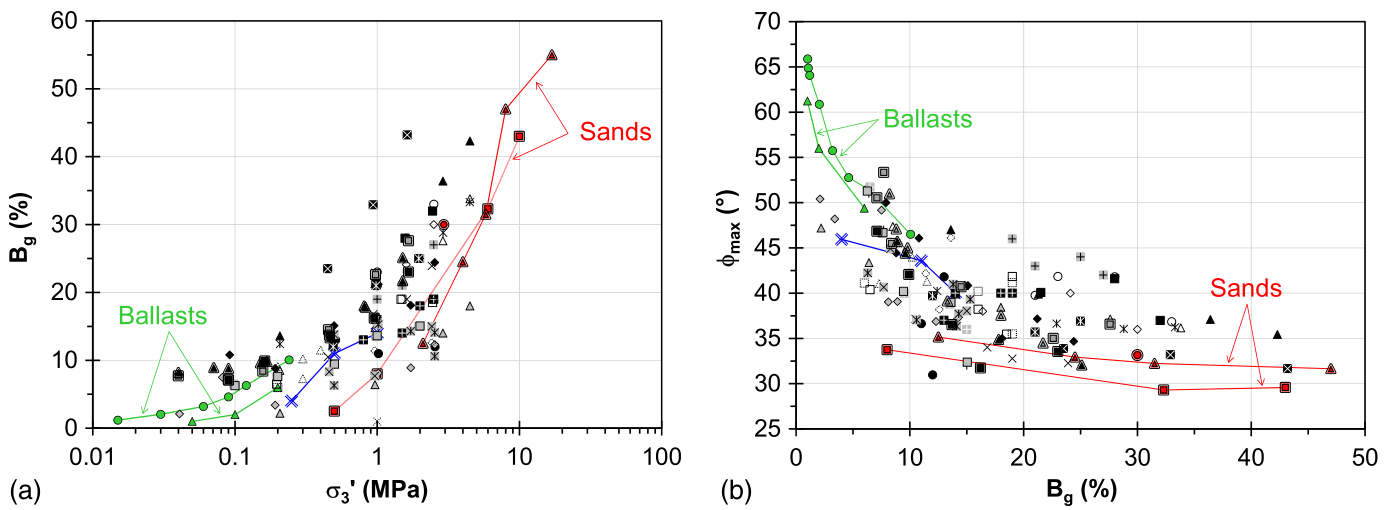
\includegraphics[width=0.8\textwidth]{figures/figure-3.png}
    \bicaption{Marsal’s breakage ratio}{Marsal破损率}
    \label{figure:3}
\end{figure}
    }

    \switchcolumn*

    It is well known that $B_g$ is expected to be inversely proportional to the initial uniformity coefficient $C_u=d_{60}/d_{10}$ \citep{Hardin19851177,Ovalle20162383}. However, it is not worth proposing a relationship for the current rockfill database given the large data scatter due to other independent variables that affect the material response.

    \switchcolumn

    众所周知,$B_g$与初始均匀系数$C_u=d_{60}/d_{10}$成反比\citep{Hardin19851177,Ovalle20162383}。然而,考虑到其他影响材料响应的自变量造成的大数据散点,对于目前的碎石数据库,提出一个关系是不值得的。

    \switchcolumn*[\biparagraph{Secant Young’s Modulus}{割线杨氏模量}]

    Young’s moduli values for rockfills have been proposed based on dam settlement analyses \citep{Hunter2003909,Kermani2018}. However, data from stress-controlled laboratory tests needed for calibration of constitutive models are scarce. Here, secant Young’s moduli from drained triaxial stress paths were obtained to compare the results with typical values used for sands. To avoid experimental scatter from data recorded at small strains in triaxial tests, a convenient modulus $E_{50}$ has been chosen, defined as the secant modulus associated with a deviatoric stress level ($q=\sigma_1^\prime-\sigma_3^\prime$) equal to half of the maximum strength. $E_{50}$ is commonly fitted by the following expression:

    \switchcolumn

    根据大坝沉降分析,提出了碎石料的杨氏模量值\citep{Hunter2003909,Kermani2018}。 但是,本构模型校准所需的应力控制实验室试验数据很少。 在这里,从排水的三轴应力路径获得了割线杨氏模量,将结果与用于砂土的典型值进行了比较。 为了避免在三轴试验中以小应变记录的数据产生实验性分散,我们选择了方便的模量$E_{50}$,定义为与偏应力水平($q=\sigma_1^\prime-\sigma_3^\prime$)相关联的正割模量,该水平等于最大强度的一半。$E_{50}$通常由以下表达式拟合:

    \CrossColumnText{
        \begin{align}
            E_{50}=K_{50} \cdot p_{a}\left(\frac{\sigma_{3}^{\prime}}{p_{a}}\right)^{n}
            \label{equation:3}
        \end{align}
    }

    \switchcolumn*

    \noindent
    where $n$ = fitted parameter, typically from 0.4 to 0.6 in sands \citep{Schanz1998383,Schanz1999281}; $K_{50}$ = reference normalized modulus; and $p_a=0.1$ MPa = reference pressure. \enautoref{figure:4} presents $E_{50}$ for all rockfill materials compared to data of dense quartzitic sands and ballasts. In addition, \enautoref{equation:1} is plotted assuming $n=0.5$ and typical values of $K_{50}$ of 200 and 400 for loose and dense sands, respectively \citep{Schanz1998383}. The comparison indicates that most rockfills have lower moduli than loose sands. By contrast, $E_{50}$ of ballasts at low pressure is similar to the values for dense sands, but tends to be in the range for rockfills at intermediate pressures of 100–200 kPa. As an explanation of this result, it is thought that even a small number of crushing events occurring in rockfill and ballast materials at relatively small strains (e.g., attrition process removing asperities) could result in a significant drop in material stiffness. At high stresses, crushing becomes significant in sands and the stiffness of sands and rockfills follows a similar trend.

    \switchcolumn

    \noindent
    其中$n$为拟合参数,通常在砂土中为0.4到0.6 \citep{Schanz1998383,Schanz1999281};$K_{50}$为参考归一化模量;$p_a=0.1$MPa为参考压力。 \cnautoref{figure:4}给出了所有碎石料的$E_{50}$与致密石英砂和石渣的数据的比较。 另外,\cnautoref{equation:1}的绘制假设$n=0.5$以及疏砂和密砂的$K_{50}$的典型值分别为200和400\citep{Schanz1998383}。 比较结果表明,大多数碎石料的模量均低于散砂。 相比之下,低压下的石渣的$E_{50}$与密砂的值相似,但在100-200kPa的中间压力下,往往处于碎石的范围内。 作为对这一结果的解释,人们认为,即使在相对较小的应变下在碎石和石渣材料中发生的少量压碎事件(例如,例如,摩擦过程消除磨损)也可能导致材料刚度的显着下降。 在高应力下,砂土的破碎变得很明显,砂土和碎石的硬度也遵循类似的趋势。

    \CrossColumnText{
        \sidebyside[verticalalignment=top][htb]{0.48\textwidth}{
    \begin{figure}[H]
        \centering
        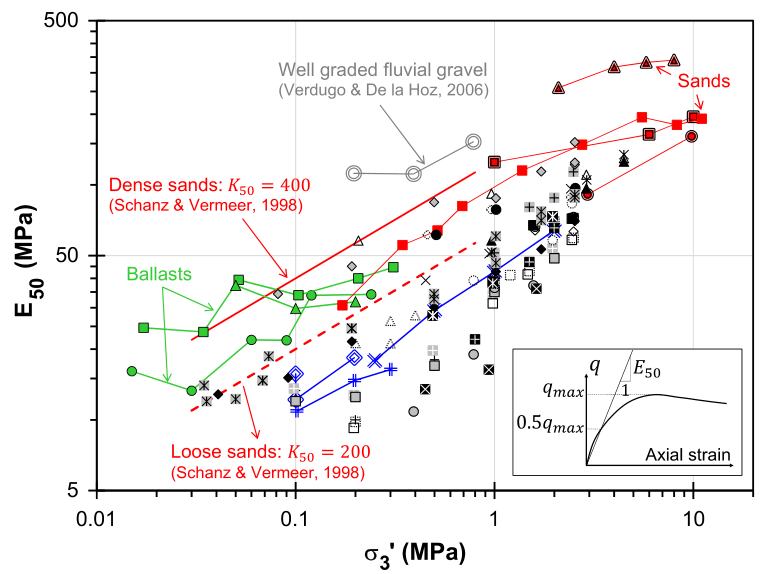
\includegraphics[width=\textwidth]{figures/figure-4.png}
        \bicaption{Secant Young’s modulus}{割线杨氏模量}
        \label{figure:4}
    \end{figure}
}{0.48\textwidth}{
    \begin{figure}[H]
        \centering
        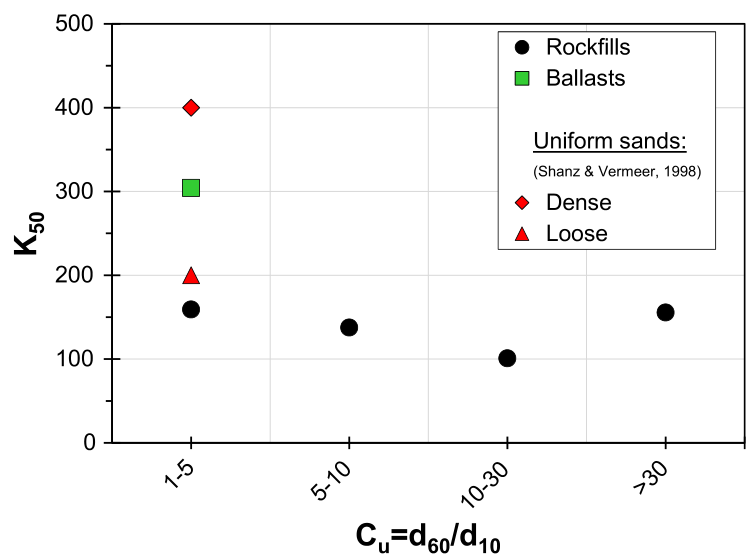
\includegraphics[width=\textwidth]{figures/figure-5.png}
        \bicaption{Normalized secant Young’s modulus}{归一化割线杨氏模量}
        \label{figure:5}
    \end{figure}
}
    }

    \switchcolumn*

    \enautoref{figure:4} also includes values of $E_{50}$ from drained triaxial tests on coarse, well-graded fluvial gravel composed of sound rounded clasts of $d_{\max}=200$ mm reported by \citet{DelaHozAlvarez2007} and \citet{Verdugo2007243}. In this case, the amount of particle crushing is considerably lower than in rockfills due to both high Cu and highly resistant rounded gravel clasts, resulting in $E_{50}$ being comparable to dense quartzitic sands.

    \switchcolumn

    \cnautoref{figure:4}还包含\citet{DelaHozAlvarez2007}以及\citet{Verdugo2007243}报道的对粗、级配良好的河流砾石进行的排水三轴试验的$E_{50}$值,这些砾石由$d_{\max}=200$毫米的良好圆形碎屑组成。 在这种情况下,由于高$C_u$和高强度的圆形砾石碎屑,颗粒破碎量要远低于碎石,使得$E_{50}$可与致密的石英砂媲美。

    \switchcolumn*

    For the data compiled here, $K_{50}$ from \enautoref{equation:3} was fitted by separating and averaging the data in ranges of initial $C_u$. As shown in \enautoref{figure:5}, regardless of the value of $C_u$, the data for rockfill are in a narrow band of $K_{50}=100–200$, typically associated with loose sands.

    \switchcolumn

    对于此处汇编的数据,请从\cnautoref{equation:3}中获取$K_{50}$。通过在初始$C_u$范围内分离和平均数据来拟合。 如\cnautoref{figure:5}所示,无论$C_u$的值如何,堆石的数据都在$K_{50}=100–200$的窄带中,通常与松散的砂土有关。
    
\end{ParaColumn}